The back-end readout card for the system under development, the Zynq UltraScale+ RFSoC ZCU216 Evaluation Card, was chosen taking into consideration the points described in \autoref{sec:selection}.
In this section, the overall architecture and features of the card are presented.
A possibility for evaluation of the card is also demonstrated.
At last, a design for the read-out firmware is proposed. 

\section{Xilinx ZCU216 Evaluation Card}
The ZCU216 Evaluation Card is equipped with the ZU49DR Zynq Ultrascale+ RFSoC \gls{rfsoc} (Gen 3). 
It allows for quick evaluation of the on-chip \gls{rf} data converters and quick prototyping of different user-defined systems.

The features which are important for the designed read-out system are listed in the following:
\begin{itemize}[noitemsep]
	\item Sixteen 14-bit, \SI{2.5}{\giga \sample \per \second} RF-ADC
	\item Sixteen 14-bit, \SI{10}{\giga \sample \per \second} RF-DAC
	\item I/O expansion options: \gls{fpga} Mezzanine Card (\gls{fmc}+) interfaces, RFMC 2.0 interfaces, and Pmod (peripheral module) connections
	\item \gls{ddr}4 \gls{dimm} – 4 GB, 64-bit, 2.666 MT/s, attached to the \gls{pl}
	\item \gls{ddr}4 \gls{sodimm} – 4 GB, 64-bit, 2.400 MT/s, attached to the \gls{ps}
	\item High-speed I/Os: 2x2 \gls{sfp}/SFP+/zSFP+/SFP28 modules
	\item Breakout cards for evaluation of the \gls{adc} and \gls{dac} performance, together with a clock add-on card for internal/external reference clocking
\end{itemize}
Other peripheral connections and features are shown in the topview of the board in \autoref{fig:zcu216}.
\begin{figure}[tbh]
	\centering
	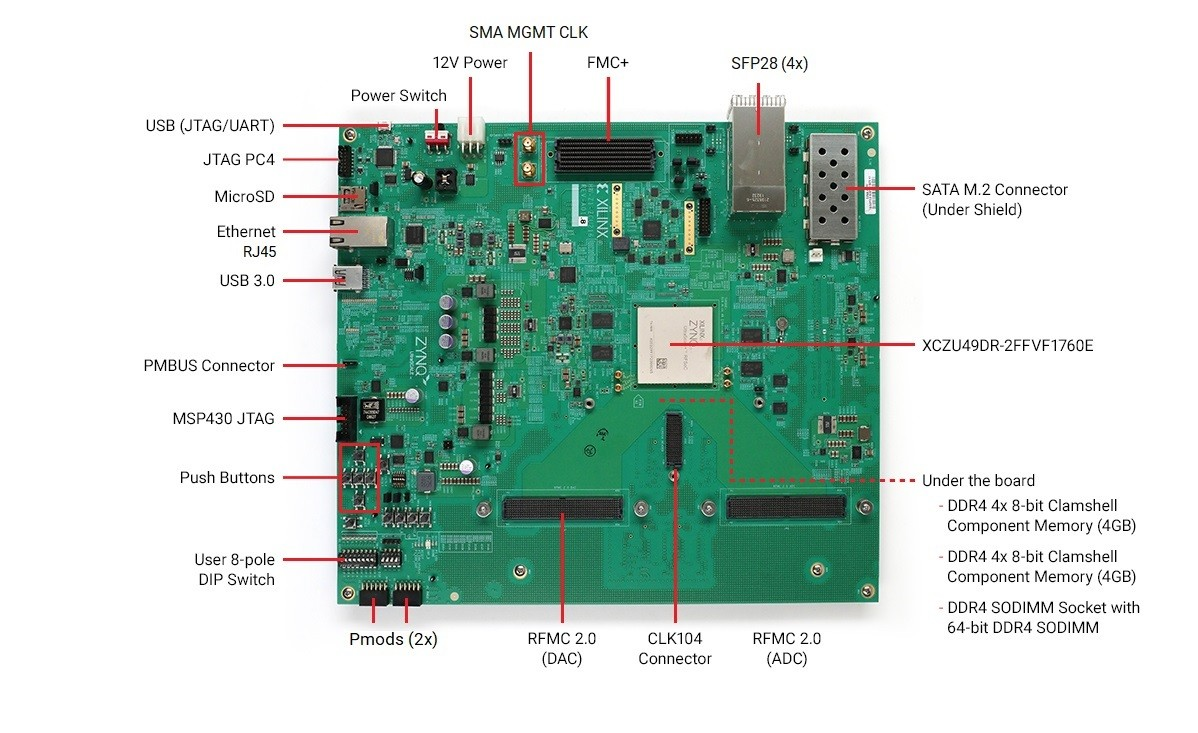
\includegraphics[width = \textwidth]{chap/04-work/img/zcu216}
	\caption{Topview of ZCU216 evaluation board with labeled components}
	\label{fig:zcu216}
\end{figure}

\paragraph{ZU49DR RFSoC}
Together with an UltraScale+ programmable logic, the ZU49DR \gls{rfsoc} integrates an Arm\textregistered Cortex\texttrademark-A53 \gls{ps}.
This \gls{ps} contains a 64-bit quad-core Arm\textregistered Cortex\texttrademark-A53, serving as \gls{apu}, and a dual core Arm Cortex-R5F, serving as \gls{rpu}.
Furthermore, the system integrates \gls{rf} data converters, allowing to use the system for \gls{rf} applications.
At the moment of writing, this is the industry's only single-chip, adaptable radio platform \cite{zu49}.
This setup allows to 
\autoref{fig:rfsoc} shows the general block diagram of the \gls{rfsoc}.

\begin{figure}[tbh]
	\centering
	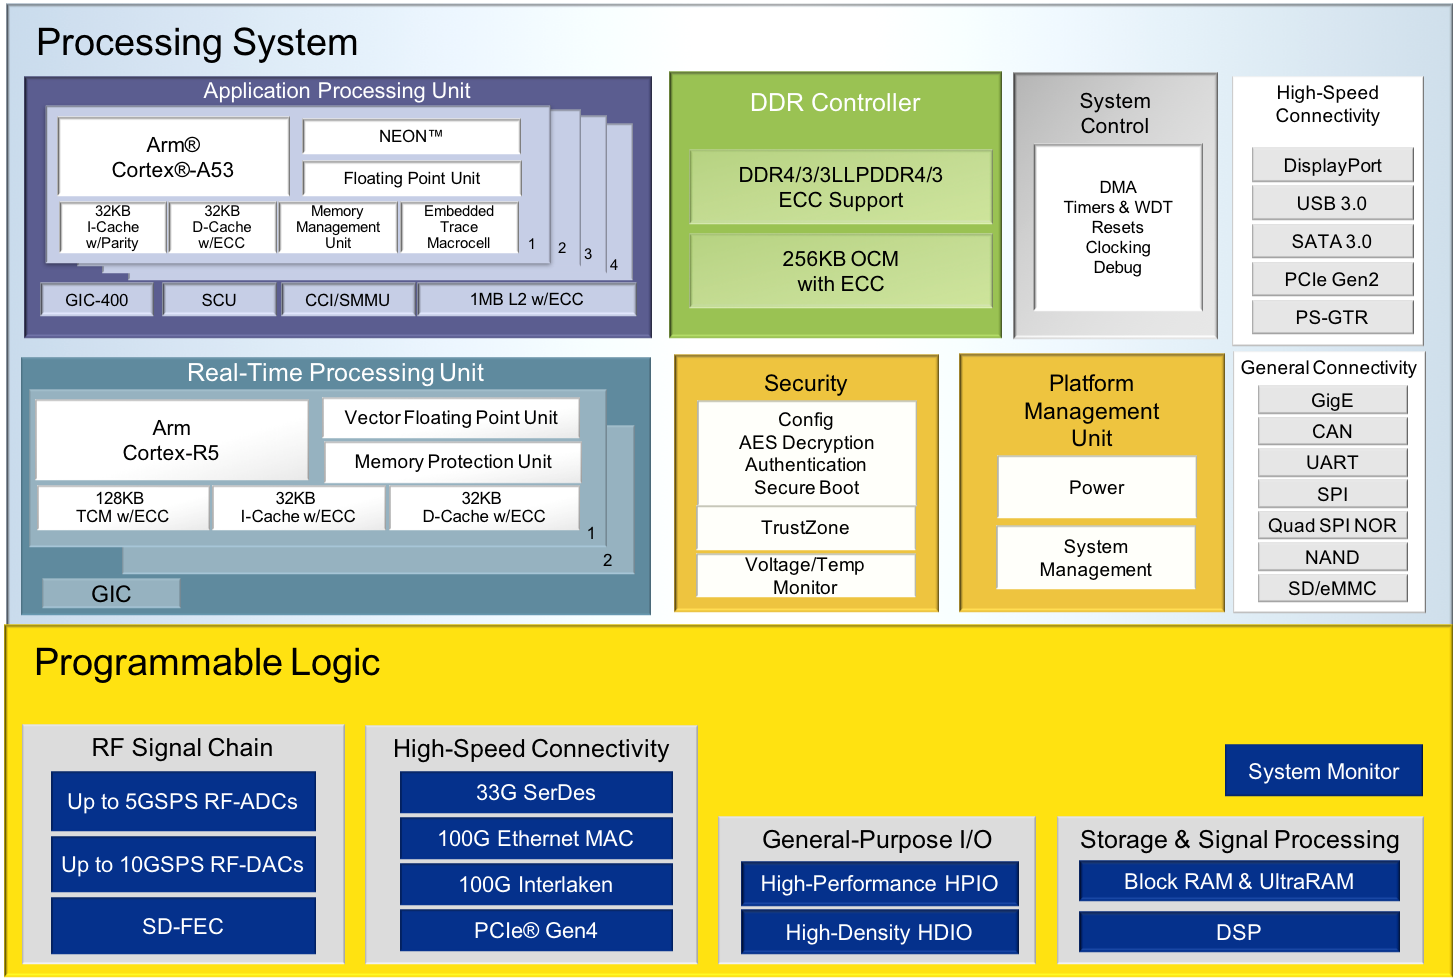
\includegraphics[width = \textwidth]{chap/04-work/img/rfsoc_blockdiagram}
	\caption[Zynq Ultrascale+ RFSoC block diagram]{Zynq Ultrascale+ RFSoC block diagram, showing in detail the different components of the \gls{ps} and \gls{pl}}
	\label{fig:rfsoc}
\end{figure}

\paragraph{Evaluation Tool}
In order to provide a quick evaluation of data converter performance an evaluation framework from Xilinx can be deployed on the card (see \autoref{fig:evalTool}). 

\begin{figure}[tbh]
	\centering
	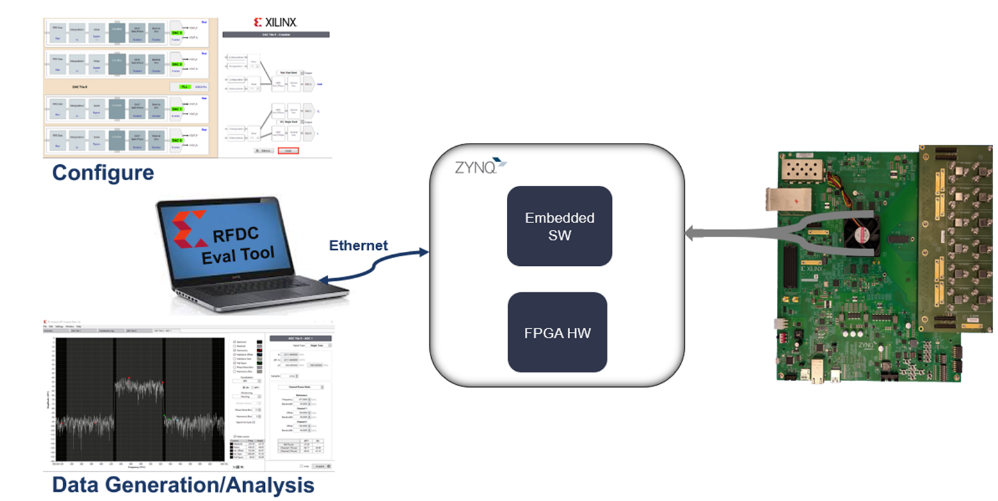
\includegraphics[width = \textwidth]{chap/04-work/img/zcu216evaltool}
	\caption[ZCU216 Evaluation Tool]{Concept of the Evaluation Tool for the ZCU216, showing the interactions between the host PC and the board}
	\label{fig:evalTool}
\end{figure}

It enables control of the ZCU216 \glspl{ip} and the associated designs from a host PC. 
With the tool, different \gls{rf} configurations can be explored, \gls{rf} data can be generated and captured and different \gls{rf} metrics (see \autoref{ssec:adc_charac}) can be observed.  
For this, the breakout card provided with the board, or any other user-designed board, needs to be attached to the evaluation card via the RFMC connectors.

The RF DC (Data Converter) Evaluation Tool consists of two parts:
\begin{itemize}
	\item Hardware design on the \gls{pl}/\gls{fpga}, in order to implement the configuration and data generation/capture of the data converters. It is built around the RF Data Converter \gls{ip} Core from Xilinx, descrived in \autoref{sec:firmware}.
	\item Software design on the \gls{ps} and host PC, in order to control the hardware implemented on the \gls{fpga}.
	On the \gls{ps} a Linux application receives commands from the host PC \gls{gui} over Ethernet. Based on the commands, it performs the according action, e.g. setting the sampling clock or enabling/disabling data converter channels. The \gls{gui} provides a convenient possibility to configure the data converters. Data generation via \glspl{dac} can be started, as well as data capture with the \glspl{adc}. Furthermore, the tool provides methods to quickly characterize the performance of the data converters (see \autoref{fig:gui}) from which the performance of the plugged break-out board can be derived.
\end{itemize}


\begin{figure}[tbh]
	\centering
	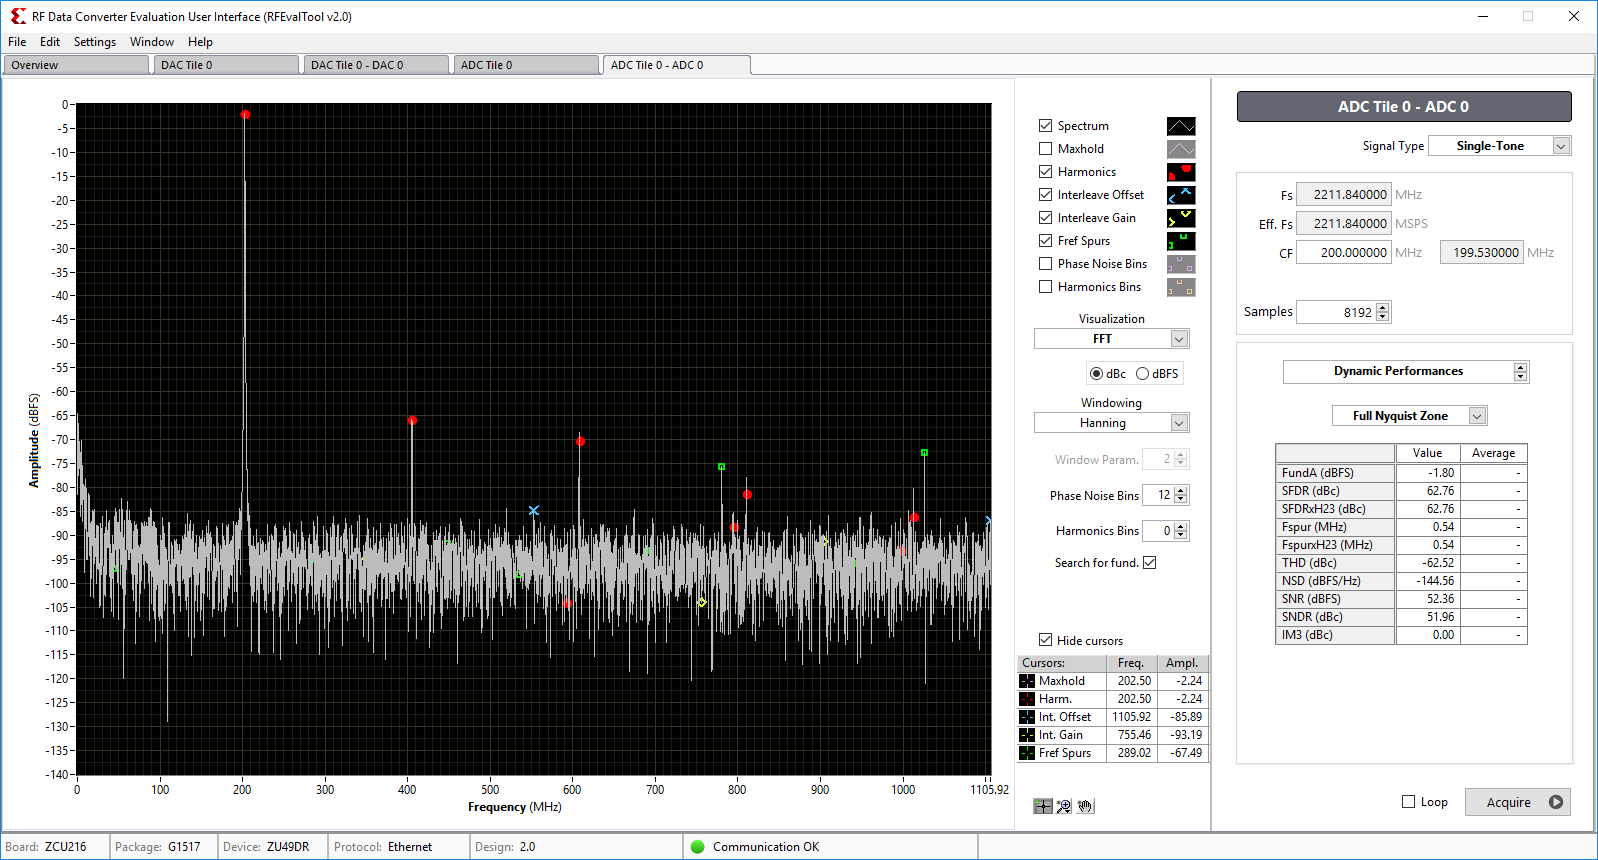
\includegraphics[width = \textwidth]{chap/04-work/img/evaltool}
	\caption{GUI of the RF Data Converter Evaluation Tool}
	\label{fig:gui}
\end{figure}

\section{Firmware}\label{sec:firmware}
Similar to the evaluation tool, the firmware for the readout system should contain a software part on the \gls{ps} which allows for control and configuration of the data converters. 
The hardware design part should implement the interface to the sampling board. 
This means it should provide the necessary interfaces to configure the data converters on the readout card, as well as slow control to the delay chips and \glspl{pll} on the sampling board (i.e. through \gls{sdi} and \gls{spi}). 
Furthermore, the high-speed data-throughput interface should be implemented.

\autoref{fig:firmware} shows the general schematic of the firmware on the readout card.
\begin{figure}[tbh]
	\centering
	\includegraphics[width = \textwidth]{chap/04-work/img/firmware.tikz}
	\caption{Schematic of the firmware and processing unit on the readout card}
	\label{fig:firmware}
\end{figure}

The sampled data is propagated from the sampling card to the \glspl{adc} inside the \gls{fpga}. 
This data is written in the \gls{ddr}, from which it is accessible by the data interface, which is responsible for the high-speed data transfer to the following processing node in the \gls{daq} system.
A built-in test-loop is implemented with an integrated \gls{dac}, in order to produce test signals which are propagated to the sampling board.
Configuration of the data converters is done via the Xilinx ``RF Data Converter'' which is described below. 

Components on the sampling board, such as the delay chips, are controlled via \gls{spi} interface. 
This interface is connected to a user bank register, where the user can specify e.g. the desired delay values.

The \gls{ps} communicates with the \gls{pl} via \gls{axi}.
\gls{axi} is a parallel, synchronous, multi-master, multi-slave communication interface.
On the \gls{ps} an operating system, e.g. Linux, or a standalone C application, can run implementing functionalities for the user to be able to control the overall system.
Access to the \gls{ps} is provided by for example via Ethernet or USB.


\subsection{Programmable Logic - Hardware design}
For synthesis and analysis of the \gls{hdl} design for the \gls{pl}, the Xilinx Vivado \gls{ide} is used.
To configure and control the data converters, the RF Data Converter IP Core from Xilinx is used.
In order to program the components on the sampling board, appropriate \gls{spi} interfaces are implemented, respecting the recommendations in the data sheet.

\subsubsection*{RF Data Converter IP Core}
In order to configure the data converters, the \gls{hdl} design should be based around the Xilinx RF Data Converter IP Core. 

\begin{figure}[tbh]
	\centering
	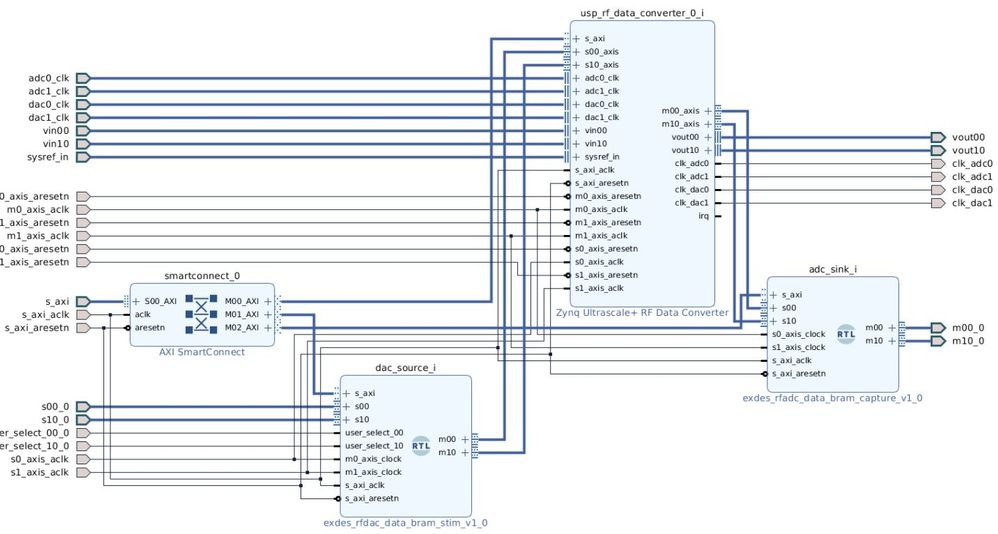
\includegraphics[width = \textwidth]{chap/04-work/img/rf_data_converter}
	\caption{Simple example design with the RF Data Converter}
	\label{fig:rf_dc_ex}
\end{figure}

\subsubsection*{Slow Control}
Components on the sampling board are controlled via a slow control interface. 
As example, the on-bard delay chips are controlled via a \gls{sdi} interface, consisting of four signals: EN, SDIN, SCLK and SLOAD. 
In order to program a certain delay, the timing diagram shown in \autoref{fig:delay_diagram} has to be respected.
The delay chip only accepts data when the EN input is HIGH. 
Therefore, this signal has to remain high in the course of the whole data transaction. 
The data pin, SDIN, which is clocked in by the SCLK signal, has to respect the following structure: delay channel select bit, mode select bit, followed by 9 data bits, which represent the desired delay value in binary format.
At the end, SLOAD has to be asserted HIGH, in order to signal the chip to load the received data into the chip's internal register.
The \gls{hdl} implementation for this interface is listed in the appendix.
\begin{figure}[tbh]
	\centering
	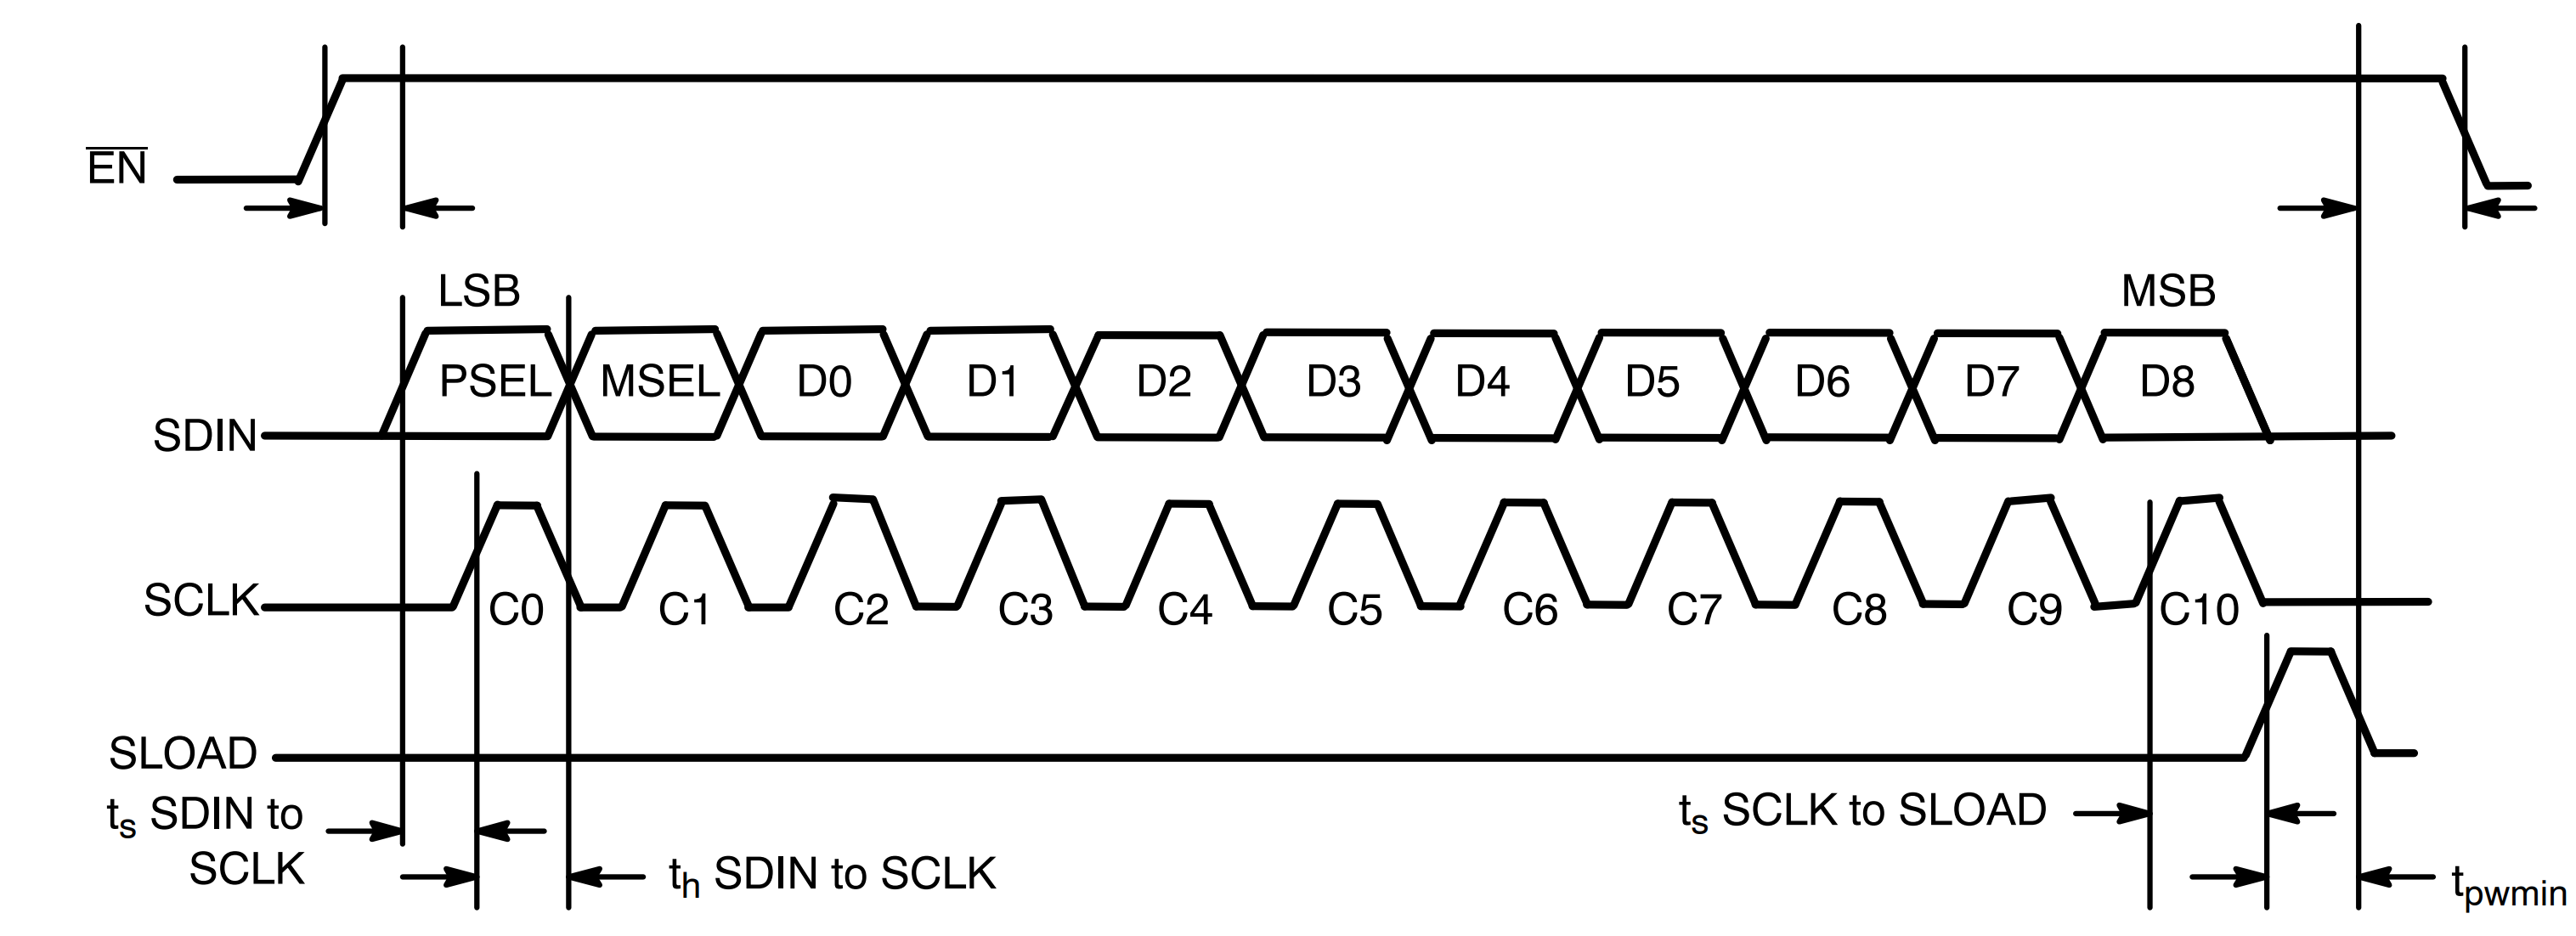
\includegraphics[width = \textwidth]{chap/04-work/img/sdi_interface_delay}
	\caption{SDI Timing diagram for the NB6L295 delay chip \cite{NB6L295}}
	\label{fig:delay_diagram}
\end{figure}
In a similar way, the interface for other components is to be implemented.

\subsubsection*{RDMA over Converged Ethernet (RoCE)}
Remote Direct Memory Access (RDMA) is a direct memory access from the memory of one computer into that of another without involving either one's operating system. This permits high-throughput, low-latency networking, which is especially useful in massively parallel computer clusters.

RoCE is a network protocol defined in the InfiniBand Trade Association (IBTA) standard, allowing RDMA over converged Ethernet network. Shortly, it can be regarded as the application of RDMA technology in hyper-converged data centers, cloud, storage, and virtualized environments. 
It possesses all the benefits of RDMA technology and the familiarity of Ethernet.

The ERNIC (Xilinx Embedded RDMA enabled NIC) IP provides an Initiator and Target  implementation of RDMA over Converged Ethernet (RoCE v2) enabled NIC functionality. This IP is specifically designed for embedded applications that require reliable transmission over Ethernet networks.



\subsection{Processing Unit - Software Design}
In order for the user to be able to control the whole system, some kind of application has to be implemented for control of the hardware design.
For this the \gls{ps} side of the \gls{rfsoc} is used. 
The Arm Cortex processor allows to implement standalone C application, as well es hosting an operating system like Linux. 
Providing a number of peripheral connections, like RJ45 or USB, the \gls{ps} can easily be accessed by the user from another host computer, given the necessary drivers and protocols are implemented.
The aforementioned evaluation tool for example uses the Linux application \textit{rftool} in order to receive commands and perform the according action.

